% Chapter Template

\chapter{Fabrication and Characterization of Polymeric Fibers through Near-Field Electrospinning} % Main chapter title

\label{Chapter:4}

\section{Materials and Methods}

\begin{figure}[!th]
\centering
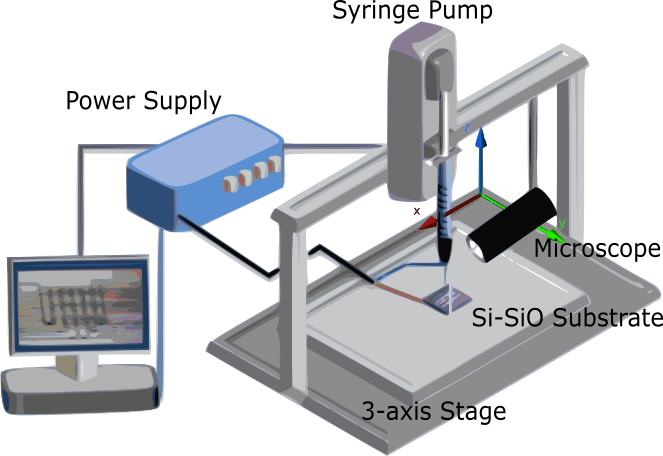
\includegraphics[scale=0.50]{./Figures/NFESsetup.png}
\decoRule
\caption[NFES experimental setup]{NFES experimental setup. Adapted from \cite{Floreshernandez2020}}
\label{fig:NFESsetup}
\end{figure}

The near-field apparatus (Figure \ref{fig:NFESsetup}) is comprised by a high voltage supply (HVS448 3000 V, LabSmith, Livermore, CA, USA), a three-axis stage, syringe pump (Pump 11 Elite, Harvard Apparatus, Cambridge, MA, USA). Samples were prepared as per the rheology measurements in Chapter \ref{Chapter:3}. Experiments were conducted with 1 milliliter slip-tip insulin syringes with 21 gauge precision tips (Nordson Engineered Fluid Dispensing, Westlake, OH, USA). The power supply and 3-axis stage are controlled through a desktop computer, while the syringe pump is controlled manually. Fiber depositions were placed on a $\textrm{Si}-\textrm{SiO}_2$ wafer. The voltage between the nozzle tip and the collector was varied between $200 [\textrm{V}]$ and $600 [\textrm{V}]$ in increments of $100 [\textrm{V}]$, keeping a constant current of $10 \mu A$. For applied voltages under $400 [\textrm{V}]$, the electric field was not strong enough to overcome the surface tension of the polymer solution and initiate the jet. To enable the fiber deposition at low voltages, the polymer jet was manually initialed by breaking the surface tension with a sharp glass tip. The working distance $L$ and stage velocity was set at a constant values for all the experiments at $0.5 mm$ and $10 mm/s$ respectively. The syringe pump was set at a steady flow rate of $0.04 \mu \textrm{L} / \textrm{min}$.

The calculated critical concentrations in Chapter \ref{Chapter:3} (Table \ref{tab:calculatedSpinnableConcentrations}) are used for the fabrication of polymeric fibers. One set of experiments was conducted for each polymer-solvent system to study the effect of applied voltage on fiber diameter. The morphology of the fibers were characterized with an optical microscope (Correct, Seiwa Optical, Dallas, TX, USA). Each sample was measured at 30+ points within the microscope field of view (Appendix \ref{Appendix_MicroscopyChar}).

\section{Results}

\begin{figure}[!th]
\centering
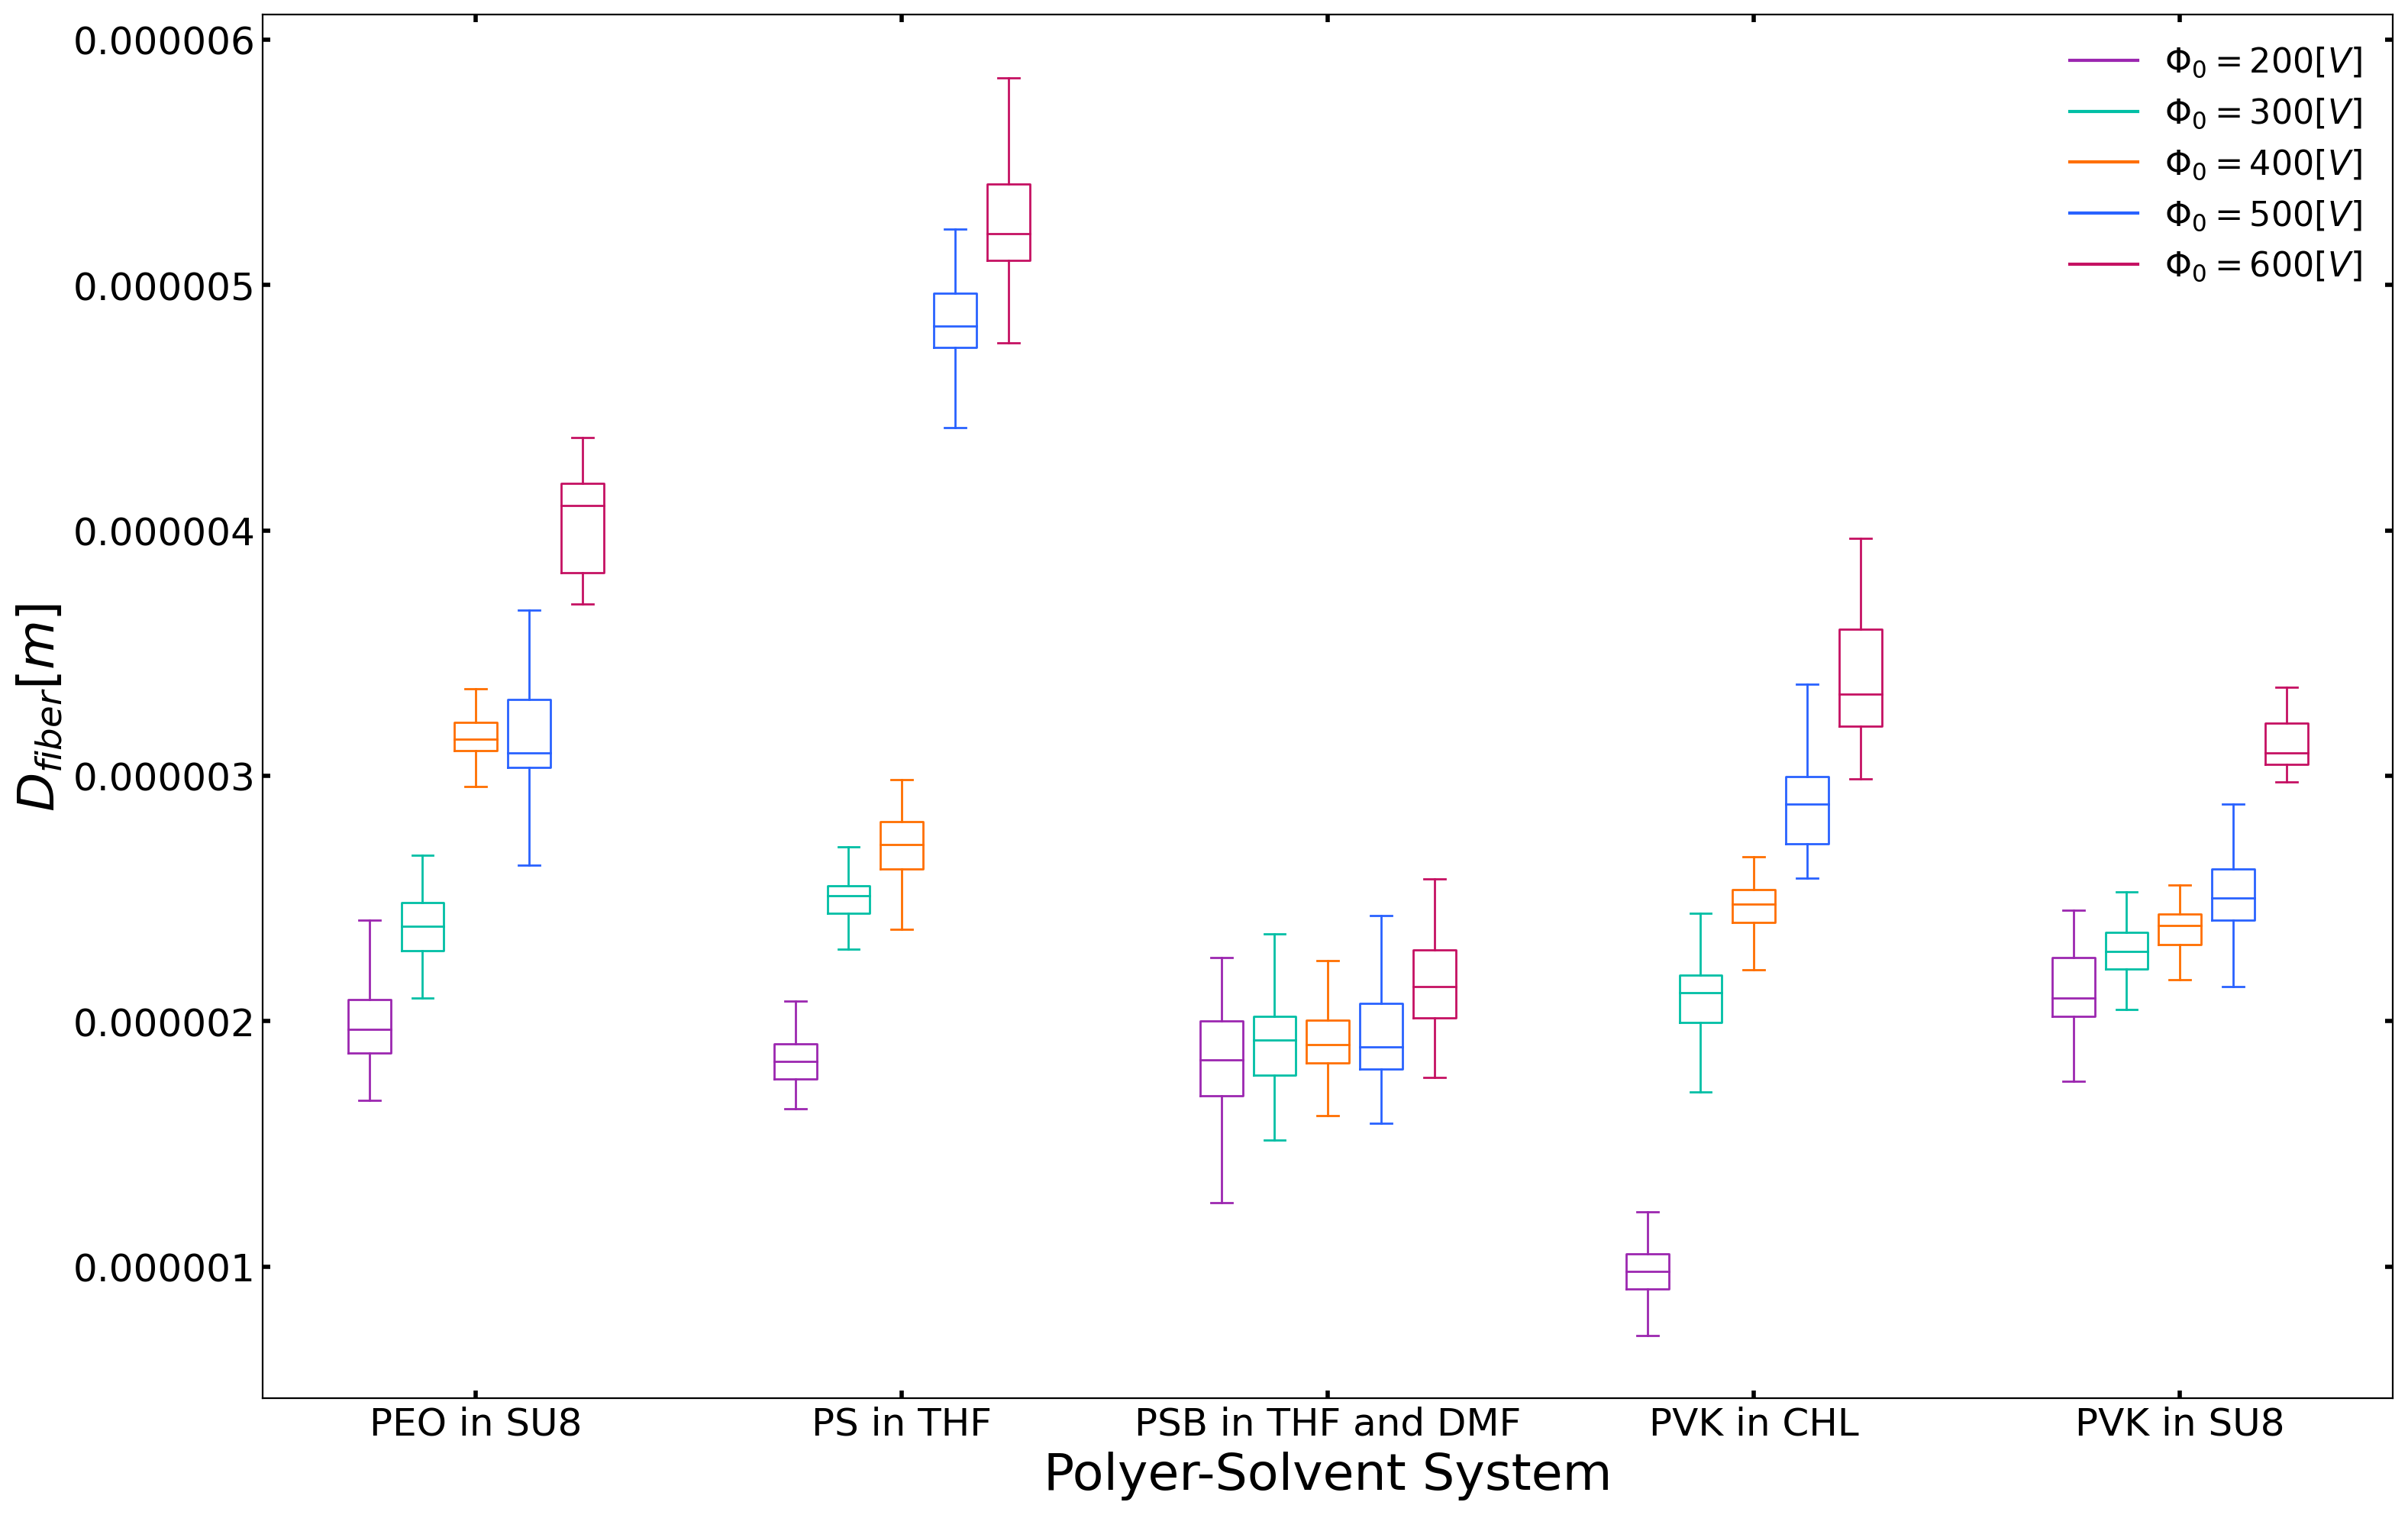
\includegraphics[width=\textwidth]{./Figures/boxplotsFiberDiameter.png}
\decoRule
\caption[Diameter of fibres for all the experiments]{Diameter of fibres for all the experiments with varing applied voltage $\Phi_0$}
\label{fig:boxplotsFiberDiameter}
\end{figure}

Figure \ref{fig:boxplotsFiberDiameter} shows a dependence of fiber diameter as a function of the applied voltage and confirms what was already noticed in the correlation matrix in Chapter \ref{Chapter:2}, as lower voltages yield fibers with thinner diameters. This results verify the electro-spinnability of oxygen-less polymers by NFES into fibers of $1 \mu m$ to $5 \mu m$ in diameter. PS presented complications during the NFES process as fibers of this polymer do not adhere onto the substrate making them prone to fracture or substrate abandonment, specially when printing fibers of thin diameters. To ease this complication the working distance $L$ can be reduced to let the fibers dry on the surface and prevent complete solidification while traveling the distance $L$. The increase in applied voltage can also help with this problem as more material is pulled out of the dispensing needle, however this two fixes will translate into thicker fibers.

The PVK and CHL system was the one that behaved with more similarity as the control sample of SU-8 and PEO. Uniform, $700 nm$ diameter fibers were achieved with PVK and CHL at the lowest voltage setting ($200 V$). Given the similarities with the control sample, PVK was choosen to replace the PEO to increase the spinnability of SU8. Therefore, the PVK in SU-8 system was tested in the same conditions as the previous experiments. Both polymers (PEO and PVK) in SU-8 yield parallel results in fiber morphology and in electrospinning preformanc. However, at high voltages, the PVK solution produced thinner fibers than those produced by the PEO solution. Moreover, as PVK does not contain any additional oxygen content in its structure, adding PVK can be a better alternative to electrospun SU-8 based fibers intended for carbonization as thinner fibers will have better opportunities to survive the pyrolysis process without breaking.

On the other hand, the polymer-solvent systems comprised by Poly(Styrene-co-Butadiene) (PSB) in 1-Methyl-2-Pyrrolidinone (NMP) and Poly(Styrene-co-alpha-Methylstyrene) (PSMS) in N,N-Dimethylformamide (DMF) were unable to yield fibers. In the case of the PSB/NMP solutions, a hard shell was formed around the polymer drop at the tip of the nozzle preventing the jet to initiate, which causes clogging. Seems that rapid volatilization of NMP is not the case as PSB was successfully electrospun with higher volatile solvents (THF and DMF). Notice that vapor pressure of NMP is around $39 \textrm{Pa}$ at $25^{\circ} C$, THF and DMF have vapor pressures of about $19.3 \textrm{kPa}$ at $20^{\circ} C$ and $0.49 \textrm{kPa}$ at $25^{\circ} C$ respectively. \cite{ICSCs} On the other hand, PSMS in DMF was not able to produce fibers as the jet was not initiated. After noticin that que calculated critical concentration $c^*$ is not spinnable the solutions of 10 and 15 $wt\%$ were also tested in the NFES apparatus with no success. The cause of the non-spinnable nature of PSMS can be laid on the fact that PSMS pellets were brittle and capable of making fine PSMS dust with ease, unlike PS and PSB pellets which have an elastic behavior.

\section{Conclusions and Future Work}

A series of experiments were carried out in order to find a correlation between the rheological properties of different polymer solutions in near-field electro-mechanical spinning for carbon structures. Flow curve measurement tests where carried out in an oscillatory rheometer to estimate the critical concentrations of various polymer-solvent systems at which they are spinnable by NFES. Since the formulation is 0.25 $wt\%$ PEO in SU-8 2002 has been studied in the past and is known to yield good polymer solutions but fails at the pyrolysis, this work intends to find spinnable and pyrolyzable systems as well as a method to discover new spinnable polymer solutions.

From the flow curve measurements, the zero-shear viscosity was estimated using the Carreau-Yassuda model. For all solutions, a shear thinning behavious was noticed. It was found that the viscosity-concentration plot is a good method to find the critical concentration at which the solution is able to produce fibers through NFES. However the method failed at calculating the spinnable concentration of PSMS. An significant takeaway is that a polymer does not have elastic properties in the pellet form, it will probably not work as a NFES polymer precursor.

Fibers were fabricated at different applied voltages for each set of solutions in order to very that in NFES fiber diameter increases with increasing applied voltage, whereas the inverse relationship is true for FFES. Other parameters such as working distance, stage velocity, nozzle diameter, flow rate were kept constant for all experiments; however, for low applied voltages the jet shall be initialed by manually breaking the polymer drop. the thickest average fiber diameter was achieved with the PS in THF system ($\Phi_0 = 600 V$, $D_{fiber} = 5.304 \mu m$) and the thinnest was $0.976 \mu m$ using the PVK in CHL system and an applied voltage of $200 V$. It was proved that attainable rehological information can be used to modify the NFES process parameters to yield the desired fiber morphology.

Moreover a data analysis was done on the NFES publications of the last 13 years to identify relationships between fiber diameter and the process parameters. For instance, it was confirmed that thin fibers are achived with los polymer concentrations, small nozzle diameters, low applied voltage, slow flow rates and high stage velocities. Also, using the collected data and the input of Helgeson's work \cite{Helgeson2007}, an dimensionless analysis was done to predict fiber diameters with easy to get parameters. Apart from the work done, this dissertation opens pending research to enable NFES for the fabrication of carbon structures. The following lists future work that could be done as a continuation of this thesis.

\begin{itemize}
\item Helgeson's model \cite{Helgeson2007} was thought to work with far-field electrospinning, hence the deviation of the NFES data from the model trend. For an accurate NFES fiber diameter prediction, the mechanical stresses introduced by the moving stage shall be considered in the model (Equation \ref{eqn:ohnesorgeNumberRelationship}). 
\item This work verifies the electro-spinnability of four new formulations, however fibers were not carbonized into carbon structures. Further work shall study the pyrolysis process of the proposed fibers to get carbon structures with good electrical conductivity. A photo-polymerization process could be introduced before pyrolyzation to increase the order of the molecules and achieve carbon with higher conductivity.
\item Near-field electrospinning solutions require specific viscosities to initialte a polymer jet. The viscosity-concentration plot is a helpful tool to estimate the critical spinnable concentration of a polymer-solvent system. However there is room for improvement as this method only considers reological data. Other methods could be adopted to better tune other process parameters such as stage velocity, and applied voltage.
\end{itemize}
